\section{Results}
This chapter shows the results of our research methods that we have used.

\subsection{Survey results}
From our survey form, we received 47 results, with all questions completed. We converted the data returned to us to a CSV (Comma-separated values) file and imported it into RStudio, as we did not want the data visualized by Google itself. From our survey we took the questions that we found the most useful and visualized them into plots. 
\begin{figure}[ht]
	\centering
	\textbf{Question: What type of network do you use for playing games?}
	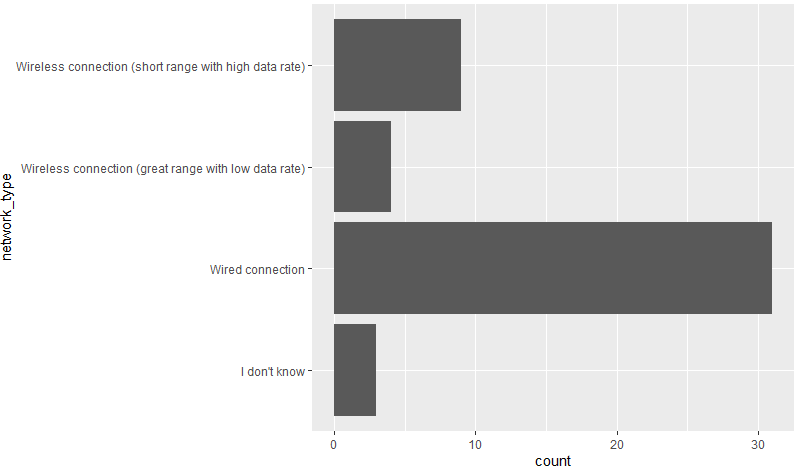
\includegraphics[width=12cm]{../img/network.png}
	\caption{The barplot shows that most people make use of a wired connection when they play games, where a few people use a wireless connection with either a great range (low data rate) or short range (high data rate)}
\end{figure}
\begin{figure}[ht]
	\centering
	\textbf{Question: Do you have a strong internet connection?}
	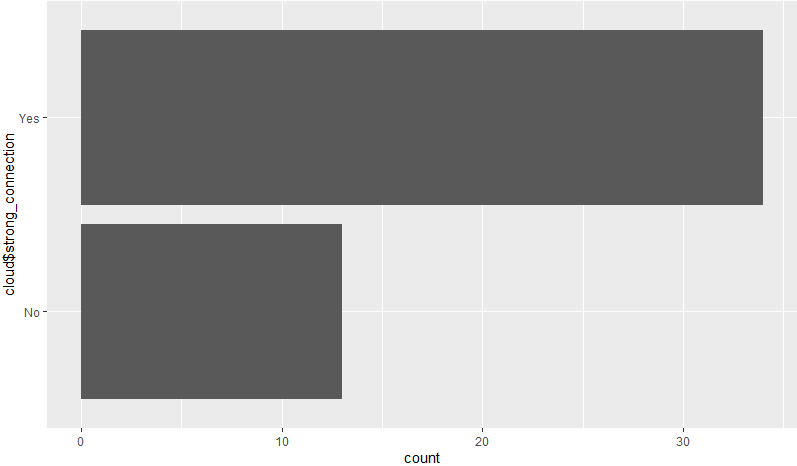
\includegraphics[width=12cm]{../img/connection.png}
	\caption{As shown in the above plot, most people claimed that they have a strong internet connection, whereas a few people have claimed that they don't have a strong internet connection.}
\end{figure}
\begin{figure}[ht]
	\centering
	\textbf{Question: When you play an online game, do you often have latency issues?}
	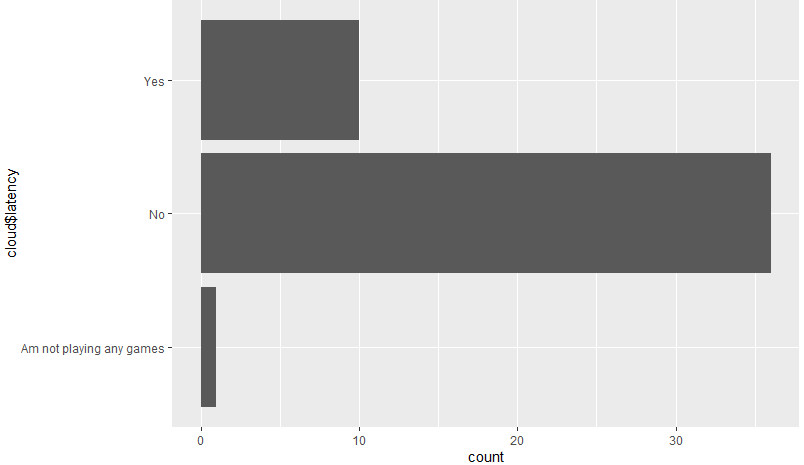
\includegraphics[width=12cm]{../img/latency.png}
	\caption{Most people said that they don't often experience latency/lag issues when they play an online game, but a few do experience latency. The people that answered "No" are most likely users of a wired internet connection, whereas the people that have said "Yes" are using a wireless connection.}
\end{figure}
\begin{figure}[ht]
	\centering
	\textbf{Question: How interested are you in cloud gaming?}
	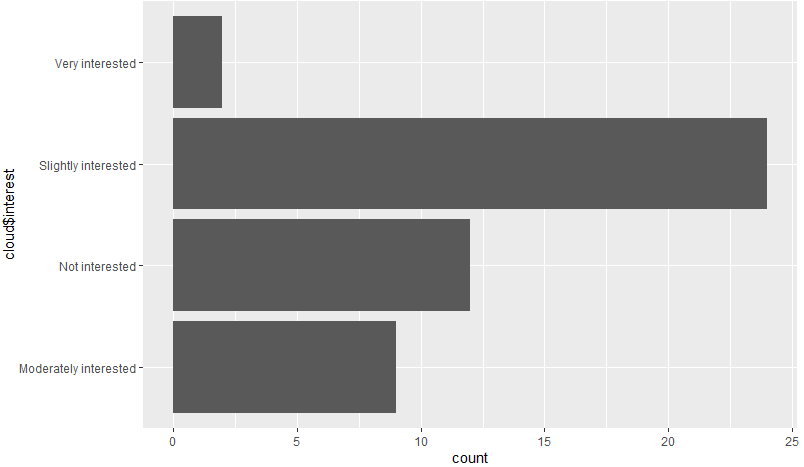
\includegraphics[width=12cm]{../img/interest.png}
	\caption{People had the choice to fill in how interested they are in cloud gaming. Most people have said that they are slightly interested in it. \\\textbf{From high to low:}\\\\
		Super interested\\
		Very interested\\
		Moderately interested\\
		Slightly interested\\
		Not interested}
\end{figure}
\begin{figure}[ht]
	\centering
	\textbf{Question: Do you think cloud gaming has a future?}
	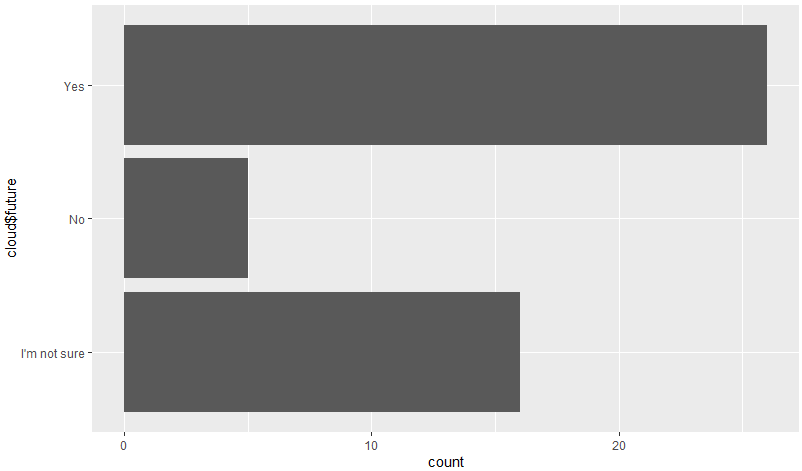
\includegraphics[width=12cm]{../img/future.png}
	\caption{Where people said that they are slightly interested in cloud gaming, most believe that cloud gaming has a future in the video game industry.}
\end{figure}
\begin{figure}[ht]
	\centering
	\textbf{Question: How likely are going to give cloud gaming a try?}
	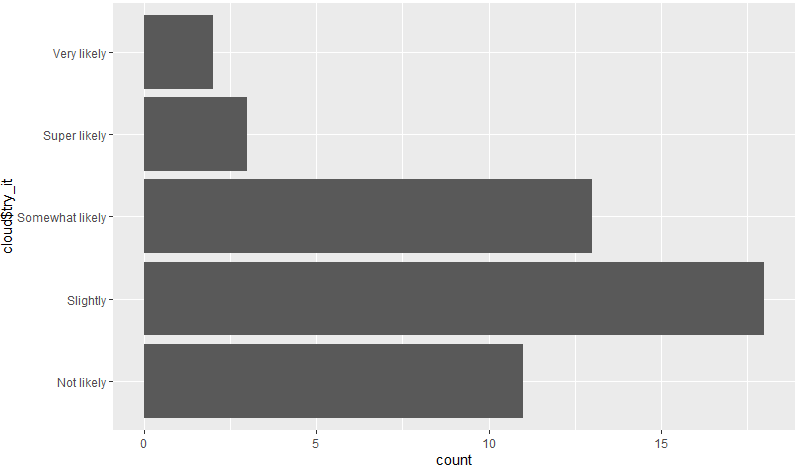
\includegraphics[width=12cm]{../img/try.png}
	\caption{Just like the question about how interested people were in cloud gaming, for this question people had the choice to fill in how likely they want to give cloud gaming a try. Just like the interest question, the most filled in answer was "Slightly". \\\textbf{From high to low:}\\\\
		Super likely\\
		Very likely\\
		Somewhat likely\\
		Slightly\\
		Not likely}
\end{figure}